\csname documentclass\endcsname[../main.tex]{subfiles}
\begin{document}
\chapter{Method}
Building on top of IntCEMs, which augment a CEM
with a greedy intervention policy model and train the two simultaneously,
we propose RLCEM,
a novel CEM model augmented with a Reinforcement Learning agent
that learns a non-greedy intervention policy.
The two are trained simultaneously, similar to IntCEM, 
where the sampled interventions are used to increase the sensitivity of the
$\mathbf{c} \to \mathbf{y}$ label prediction model.
In this chapter, we document how we propose 
to learn such a non-greedy intervention policy.
We first
formalize interventions and intervention policies,
then introduce the surrogate models we use
to calculate rewards,
and finally, present how Reinforcement Learning is used 
to learn a non-greedy intervention policy.
\section{Interventions}
A key advantage of using CBMs is having access to 
run-time interventions, which is the idea of utilizing professionals
to modify incorrect concept predictions to improve the 
performance of the model.
For simplicity, we do not consider incorrect interventions, 
i.e. when the professionals misjudge and modify
 the predicted concepts to incorrect values,
and assume that
all interventions are correct. To formalize interventions, we define
them via the following function, where
the predicted concepts $\hat{\mathbf{c}}$ and the true concepts $\mathbf{c}$ are interpolated
using a multi-hot encoding intervention vector $\bm{\mu}$.

\[I(\hat{\mathbf{c}}, \mathbf{c}, \bm{\mu}) = 
\bm{\mu} \; \mathbf{c} + (1 - \bm{\mu}) \; \hat{\mathbf{c}} \qquad \hat{\mathbf{c}}, \mathbf{c}, \bm{\mu} \in \{0, 1\}^k\]

Figure~\ref{fig:interventions} demonstrates how an intervention
is formed using 
a binary mask $\bm{\mu}$ from the predicted concepts $\hat{\mathbf{c}}$ and the true concepts $\mathbf{c}$.

\begin{figure}[!h]
    \centering
    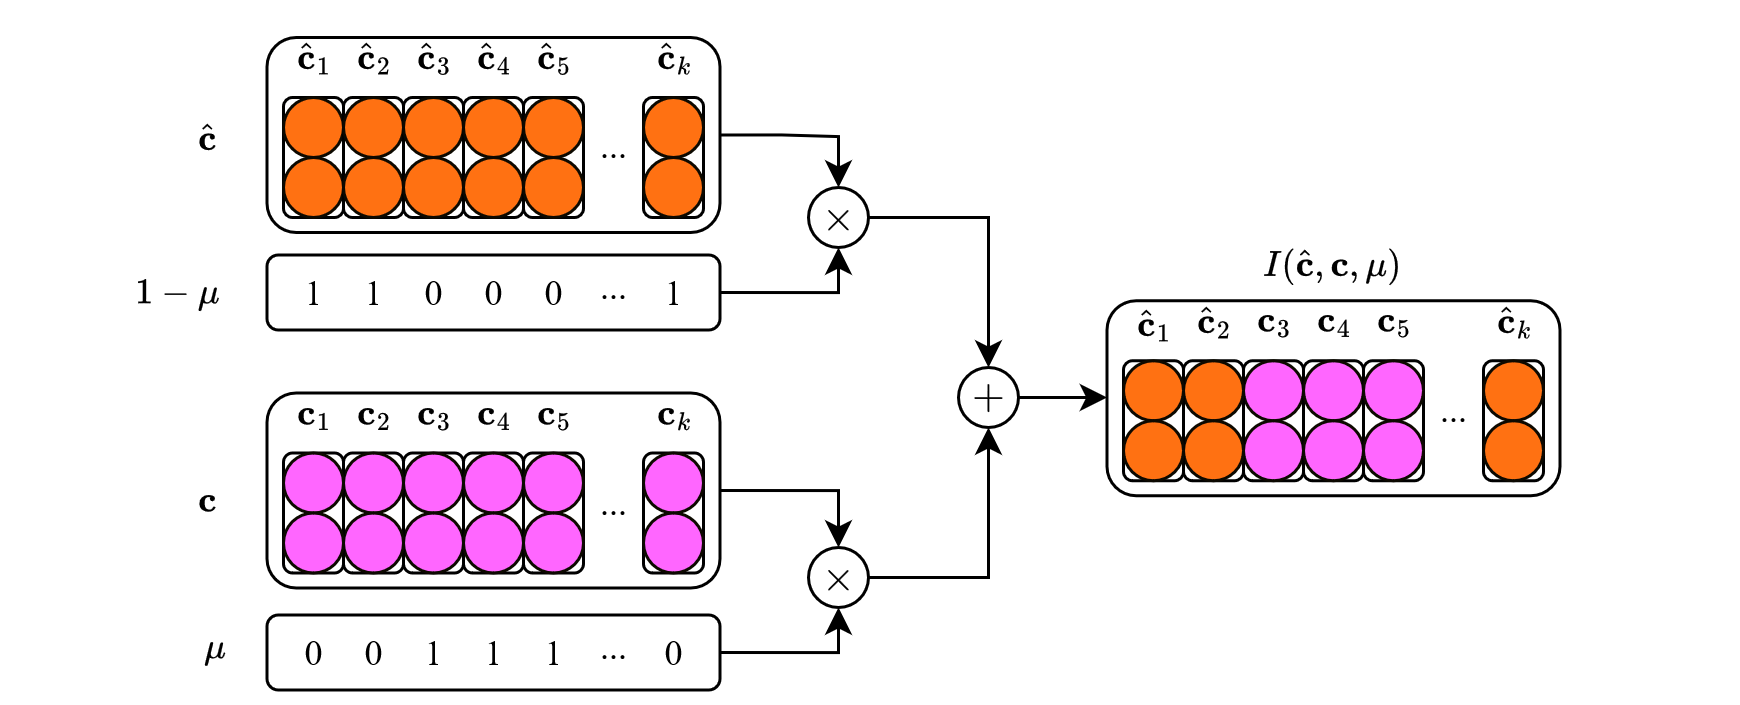
\includegraphics[width=\textwidth]{figs/method/interventions.png}
    \caption{A figure of how interventions are formed using binary masks.}
    \label{fig:interventions}
\end{figure}

\subsection{Intervention Policies}

An intervention policy $\mathcal{P}$ determines the order of concepts to intervene 
on with the goal of maximizing the accuracy of the $\mathbf{c} \to \mathbf{y}$ concept prediction model.
A greedy intervention policy is thus a collection of functions $\mathcal{P}_i$, each
of which outputs the concept to intervene on at step $i$. An optimal greedy policy is the following
\[\hat{\mathcal{P}} = \bigcup_{i=1}^k \mathop{\mathrm{argmax}}_{\mathcal{P}_i} Acc(\hat{g}(\hat{\mathbf{c}}_{\mathcal{P}_j}), \mathbf{y}) \]
% \[\hat{\mathcal{P}} = \mathop{\mathrm{argmin}}_{\mathcal{P}} \sum_{j = 1}^{k} L_{\text{task}}(\hat{g}(\hat{\mathbf{c}}_{\mathcal{P}, j}), \mathbf{y}) \]
\[\hat{\mathbf{c}}_{\mathcal{P}_0} = \hat{\mathbf{c}}, \hat{\mathbf{c}}_{\mathcal{P}_j} = I(\hat{\mathbf{c}}_{\mathcal{P}_{j-1}}, \mathbf{c}, \mathcal{P}_j(\hat{\mathbf{c}}_{\mathcal{P}_{j-1}}))\]
Which maximizes the accuracy at each step $j$ sequentially
for all $k$ concepts. At each
step, $\hat{\mathbf{c}}_{j-1}$ is 
the predicted concept after the previous $j-1$ interventions,
and we aim to maximize the accuracy of the $\hat{g}: \mathbf{c} \to \mathbf{y}$ model
on the intervened concepts $\hat{\mathbf{c}}_{\mathcal{P}_j}$ and the label $\mathbf{y}$.


Compared to a greedy intervention policy, a non-greedy intervention 
policy outputs a set of concepts to intervene on for a given budget $j$,
which we want to maximize the accuracy of the 
label predictor model on. An optimal non-greedy policy maximizes the following
\[\hat{\mathcal{P}} = \mathop{\mathrm{argmax}}_{\mathcal{P}} \sum_{j=1}^k Acc(\hat{g}(\hat{\mathbf{c}}_{\mathcal{P}_j}), \mathbf{y}) \]
\[\hat{\mathbf{c}}_{\mathcal{P}_j} = I(\hat{\mathbf{c}}, \mathbf{c}, \mathcal{P}(\hat{\mathbf{c}}, j))\]

Note that the notion of a budget, defined as the number
of concepts the model is allowed to intervene on for simplicity, is only
important for non-greedy policies. Non-greedy policies aim
to maximize the accuracy of the $\mathbf{c} \to \mathbf{y}$ model after using up the intervention budget,
and may select different sets of intervention concepts 
for different budgets. Greedy policies always select the same
concepts per step and thus the budget does not 
affect the concept selected by the policy.

% Budget
% In this project, we utilize Reinforcement Learning

\section{Surrogate Models}\label{method:surrogate}

We use generative surrogate models to model the probabilities of concepts which is used
to guide the RL model. 
Such a surrogate model is needed because
when we are using RL to learn 
a non-greedy policy, the reward, measured by the accuracy
of the model after all interventions, is returned after the final step,
if we were to reward the RL agent in the intermediate steps
this would become a greedy policy. However, previous studies have shown that
using delayed rewards, where the agent is only rewarded only
at termination after long episodes,
can pose a challenge to its learning as the agent struggles to learn
which actions lead to what consequences and what
rewards~\cite{ steps-towards-ai, temporal-credit-assignment},
and thus struggles to learn to make the correct decisions.
Therefore there is a need to introduce intermediate rewards 
to guide the RL agent to make the correct intermediate
interventions that lead 
to the largest accuracy at the end.

Following Li et al.~\cite{afa} which uses Reinforcement 
Learning
in the similar problem of Active Feature Acquisition, we use a surrogate model 
to model
the conditional probabilities $p(\mathbf{c}_u \mid \mathbf{c}_o, \mathbf{y})$, 
where $\mathbf{c}_u$ is a set of un-intervened
concepts, $\mathbf{c}_o$ a set of intervened concepts,
and $\mathbf{y}$ is the label. We select a variant of the popular normalizing flow models~\cite{normalizing-flows},
namely Arbitrary Conditional Flow (AC Flow)~\cite{acflow}
models as our generative surrogate models, 
which are flow models augmented to model arbitrary conditional probabilities of sets of variables $\mathbf{c}_u$ and $\mathbf{c}_o$.
While these AC Flow models are used to model the likelihoods
$p(\mathbf{c}_u \mid \mathbf{c}_o)$, they can easily be extended to model the class-conditional
likelihoods
$p(\mathbf{c}_u \mid \mathbf{c}_o, \mathbf{y})$. To represent
these sets of concepts while keeping the input of constant size,
the entire concept vector $\mathbf{c}$ is passed in alongside
binary masks $b$ and $m$, used to represent the concepts we are interested in. $\mathbf{c} \cdot b$ gives us 
the set of concepts $\mathbf{c}_o$ represented as a vector,
and $\mathbf{c} \cdot m$ gives us 
the set of concepts $\mathbf{c}_o$ represented as a vector
\[\mathbf{c}_o = \mathbf{c} \cdot b\]
\[\mathbf{c}_u, \mathbf{c}_o = \mathbf{c} \cdot m\]
\[\mathbf{c}_u = \mathbf{c} \cdot (1 - b) \cdot m\]
While the mask $b$ represents
the already intervened concepts, the mask $m$ represents
the missing concepts, which are concepts we are not interested
in yet. During an intervention, if the currently
already intervened concepts are $\mathbf{c}_o$,
and we want to learn about the next concept to intervene
$\mathbf{c}_u$, then the rest of the concepts 
will be masked out using $m$ as they are not of concern.

\subsection{Latent Distribution}

As described in Section~\ref{background:flow}, 
normalizing flow models utilize the change of variable formula to model probabilities,
which can be extended to include conditional probabilities. AC Flow models are built on top of
Transformation Autoregressive
Networks~\cite{tans} (TANs), and learn to model 
the probabilities for an arbitrary set of variables $p_C(\mathbf{c}_0,\ldots, \mathbf{c}_n \mid \mathbf{y})$,
modelling the underlying latent distribution using an autoregressive approach with Recurrent
Neural Networks (RNNs)~\cite{rnn}. The RNN learns to model the likelihood of 
$p_Z(\mathbf{z}_0, \ldots, \mathbf{z}_n \mid \mathbf{y})$ by sequentially processing each of the variables $\mathbf{z}_i$.
At each step, the output of the RNN $\mathbf{h}_i$ is 
passed through a learnable linear layer to get parameters for an underlying Gaussian Mixture Model (GMM),
a mixture of $K$ different Gaussian distributions~\cite{gmm}.
This allows us to compute $p(\mathbf{z}_0, \ldots, \mathbf{z}_n \mid \mathbf{y})$ 
using a weighted
sum of the probability density of the $K$ Gaussian distributions. Experimentally
we find that setting the number of components $K$ to be the number of classes 
$\mathbf{y}$ can take, which is equivalent to using one Gaussian distribution per 
class 
achieves
a good balance between model performance and computational efficiency,
which is discussed further in Section~\ref{eval:surrogate}.
While using a GMM does not directly gives us the probability
$p_Z(\mathbf{z}_0, \ldots, \mathbf{z}_n \mid \mathbf{y})$, it allows us to compute the probability density of the distribution, giving 
us the conditional likelihood of the set of variables $\mathbf{z}_0, \ldots, \mathbf{z}_n$, which provides valuable information
to the RL agent, and also allows us to sample from the distribution.

\subsection{Transformations}
In order to transform latent likelihoods $p(\mathbf{z}_0, \ldots, \mathbf{z}_n \mid \mathbf{y})$ to 
the concept likelihoods in our data
$p(\mathbf{c}_0,\ldots, \mathbf{c}_n \mid \mathbf{y})$, we
utilize a set of transformations with learnable parameters that 
map input variables $\mathbf{c}_i$ to latent variables $\mathbf{z}_i$. We follow the 
set of conditional transformations defined by Li et al.~\cite{acflow}, extend them to
be label $\mathbf{y}$ specific, and implement them.
These transformation $q_{\mathbf{c}_o, b, \mathbf{y}}$ are
conditional on 
observed concepts $\mathbf{c}_o$, binary mask $b$, and label $\mathbf{y}$, 
and are invertible so that we can obtain the liklihood and 
sample from the latent distribution. 
For all un-observed concepts $\mathbf{c}_i$,
the transformation maps them to a latent variable $q_{\mathbf{c}_o, b}(\mathbf{c}_i) = \mathbf{z}_i$. 
We can then apply the change
of variable theorem with a conditional extension, and using
the Jacobian determinant tells us how much the likelihood changes~\cite{normalizing-flows}

\[p(\mathbf{c}_u \mid \mathbf{c}_o, b, y) = \left | 
\mathop{\mathrm{det}} \frac{d q_{\mathbf{c}_o, b}}{d \mathbf{c}_u}
\right | p(q_{\mathbf{c}_o, b}(\mathbf{c}_u) \mid \mathbf{c}_o, b, y)\]

In the AC Flow model, we mainly leverage
linear transformations, where we use a MultiLayer Perceptron (MLP)~\cite{feedforward} $\phi$ to learn 
to output a weight matrix $\mathbf{W}$ and bias vector $\mathbf{t}$
\[\mathbf{W}, \mathbf{t} = \phi(\mathbf{c}_o, b, \mathbf{y})\]
As shown in Figure~\ref{fig:linear-transformation},
this gives us a linear transformation for all possible concepts,
and by indexing $\mathbf{W}_{u} = W[1-b][1-b], \mathbf{b}_{u} = \mathbf{b}[1-b]$
to select the entries corresponding to the rest of the concepts, we obtain
$\mathbf{c}_u = \mathbf{W}_{u}z_u + \mathbf{b}_{u}$. This transformation is 
straightforward to invert, and we can find the Jacobian determinant easily and apply the change of variable
theorem illustrated above to get the probability $p(\mathbf{c}_u \mid y)$.
Other variants, such as using an RNN to learn a linear transformation
for each , are also included to add flexibility to the transformations such that
we are able to model the input data distribution. More details on the transformations
 and how to find their Jacobian determinant can be found at~\cite{tans}.

These tranformations and the latent distribution are both learnt to
 model the conditional likelihoods $p(\mathbf{c}_0, \ldots, \mathbf{c}_n \mid \mathbf{y})$.
This can then be used to compute the arbitrary conditional likelihood $p(\mathbf{c}_u \mid \mathbf{c}_o, \mathbf{y})$
which is the likelihood of
seeing a set of unobserved concepts $\mathbf{c}_u$
given a set of observed concepts $\mathbf{c}_o$ and a class $\mathbf{y}$. 
By using Bayes' theorem, we note that
\[p(\mathbf{c}_u \mid \mathbf{x}_o, \mathbf{y}) = \frac{p(\mathbf{c}_u, \mathbf{c}_o \mid \mathbf{y})}
{p(\mathbf{c}_o \mid \mathbf{y})}\]
Which the right hand side terms can be computed using the AC Flow model, with
$p(\mathbf{c}_o \mid \mathbf{y}) = p(\mathbf{c}_o \mid \emptyset, \mathbf{y})$, where we 
pass in an empty set of concepts as the condition.
Due to the invertible property of the learnt transformations,
a model learnt this way also allows us to sample from the underlying probability 
distribution then applying the transformations, which gives us 
samples from the input distribution.
This is useful for the RL agent to
determine interventions as
this provides information on which concepts are likely to be present 
(or not present) given the currently intervened
concepts.
In general, we follow the advised hyperparameters from Li et al.~\cite{acflow}
for building the transformations used in our AC Flow model. This includes the rank of the linear
matrices $W$ and the hidden dimension of the latent distribution RNN. However, we notice that while
they use $n \times k$ components in the Gaussian Mixture Model where $n$ is the number of concepts
and $k$ is the number of classes, we can use $n$ components without any noticeable performance drop. 
The main power of how the AC Flow model is able to model the data distributions accurately
is via sufficient transformations, and thus we do not change them.

\subsection{Training the Surrogate Models}\label{method:training-surrogate-model}

In this project, we adapt AC Flow models to model the probabilities of concepts in CEMs during interventions.
We follow the description of Li et al.~\cite{afa} and implement corresponding AC Flow models to model
the distribution of concepts.

We train the AC Flow models using a combination of two losses, a negative
log likelihood loss and a mean-squared error (MSE) loss . 
Since these models output likelihoods directly,
we can directly maximize the likelihood, or equivalently minimizing the negative log likelihood.
Additionally, a cross entropy loss is incorporated to help the model
learn the conditional likelihood with respect to the label $y$. 
Given $\mathbf{c}_u, \mathbf{c}_o, y$, we compute the class with the highest likelihood
$\hat{y} = \mathop{\mathrm{argmax}}_y p(\mathbf{c}_u, \mathbf{c}_o \mid y)$ and compute 
a cross entropy loss $CE(\hat{y}, y)$ such that the model learns to 
output higher likelihoods for concepts that belong to the correct class.
The loss thus becomes
\[Loss = - \log p(\mathbf{c}_u \mid \mathbf{c}_o, \mathbf{y}) +
 CE(\mathop{\mathrm{argmax}}_\mathbf{y} p(\mathbf{c}_u, \mathbf{c}_o \mid \mathbf{y}),  \mathbf{y})
\]
Additionally, we add a penalty term to the loss to prevent 
the model from outputting large values of likelihoods in general.
To penalize
large values, similar to a L2 regularization loss,
we use the square of the logits for $\log p(\mathbf{c}_u, \mathbf{c}_o \mid \mathbf{y})$ and 
$\log p(\mathbf{c}_o \mid \mathbf{y})$. The effects and reasoning of this term is further discussed in 
Section~\ref{eval:surrogate-model}. The final loss for training the
AC Flow model is
\begin{align*} 
Loss = & - \log p(\mathbf{c}_u \mid \mathbf{c}_o, \mathbf{y}) + 
CE(\mathop{\mathrm{argmax}}_\mathbf{y} p(\mathbf{c}_u, \mathbf{c}_o \mid \mathbf{y}),  \mathbf{y})
\\ & + \lambda_{l2} \left ( \log^2 p(\mathbf{c}_u, \mathbf{c}_o \mid \mathbf{y}) + 
\log^2 p(\mathbf{c}_o \mid \mathbf{y}) \right )
\end{align*}


\section{RLCEM}\label{method:rlcem}

% Talk about how the RLCEM model is formed
% The goal, losses etc
% Detailed description of what happens during training and testing
% Diagram
% Talk about design choices: num_rollouts, batch_size sampling of budget etc
Instead of using CBMs as our base models, as CEMs have been shown to have
better performance with and without interventions compared to CBMs, and its 
robustness to concept-incompleteness, which is when the concepts present 
in the dataset annotations do not contain all possible concepts, we utilise CEMs
as our base model.

RLCEM is a CEM augmented with an RL agent, and is the main focus of this project.
We construct RLCEMs according to the description below, which is then compared
against the current best performing model for interventions IntCEM. The two models 
are evaluated on the datasets described in~\ref{method:datasets} and we report
the intervention performance.

\subsection{Reinforcement Learning}\label{method:rl}


We model the problem of finding a non-greedy intervention policy as a 
Reinforcement Learning problem. As mentioned in Section~\ref{background:rl},
Reinforcement Learning is used to find non-greedy solutions to problems
by design as it models the long-term effects of its actions, and aims to 
maximize the overall reward gain. 

In order to formulate the problem
as a Reinforcement Learning problem, we model the problem
of deciding the concepts to intervene on  
as a Markov Decision Problem~\cite{rl-mdp}.

\begin{itemize}
    \item States are the observations, including all the information that is available
    at each step. This contains the remaining budget and 
    state of the CEM, including its bottleneck and predicted concepts.
    This also contains the output of the surrogate model, 
    including the sampled most likely un-intervened concepts 
    $\bar{\mathbf{c}_u} \sim p(\mathbf{c}_u \mid \mathbf{c}_o, \mathbf{y})$
    $\bar{\mathbf{c}_u} \sim p(\mathbf{c}_u \mid \mathbf{c}_o)$, sampled from
    both the class-specific likelihoods and the marginalized likelihood
    as described in Section~\ref{method:surrogate}.
    \item An action corresponds to intervening on a concept out of all possible concepts.
    For simplicity, we split concepts into concept groups, and each action intervenes on all concepts
    within a concept group. This is further discussed in Section~\ref{method:datasets}.
    \item The rewards of each step is given by the increase in 
    information to the target variable $y$, $H(y \mid x_o) - \mathbb{E} [H(y \mid x_u, x_o)]$. This information
    is directly obtained from the AC Flow surrogate model. When the entire intervention sequence finishes,
    or when we reach the termination state where the budget is insufficient for more interventions,
    the final reward is the negative of the Cross Entropy Loss of the predicted label with respect to the 
    true label, where a higher value corresponds to 
    a lower discrepancy between the prediction and the true value. This corresponds with the goal of 
    maximizing accuracy after a set number of interventions. As this requires knowledge of the true label,
    this reward is only computed during training for computing the loss
    and is not accessible to the model during testing. This is also the reason why
    Reinforcement Learning is unable to learn a greedy intervention policy as this would
    require knowledge of the ground truth label at each step to compute the reward.
    \item The sequence reaches the termination state when the entire budget has been consumed.
    
\end{itemize}

% In order to decide when to terminate, 
% To model the budget and costs for the interventions, we come up with two approaches:

\begin{enumerate}
    \item Incorporate the acquisition costs for each concept into the reward by subtracting
    the corresponding cost. Thus the RL agent
    learns to balance automatically intervening on concepts that are more costly versus the
    potential extra reward gained by the increase in information and accuracy. The RL agent then determines when to terminate
    if the cost of intervening on new concepts outweight the potential gain.
    \item Only utilize the information gain in each step to determine 
    
\end{enumerate}

We end up choosing the second approach. After utilizing the first approach,
we found it difficult to balance the weight of costs versus the other rewards, and 
it increases the hyperparameters we have to tune, and allowing the RL agent to decide 
when to terminate the intervention process does not really work for intervening with budgets.
This is because 

To simplify the problem, we assume that all concept groups have the same cost
to intervene on. Thus we set the cost of each intervention to be 1, and the budget
becomes the number of possible interventions.

\subsection{Comparison with Active Feature Acquisition}

In Active Feature Acquisition as described in Section~\ref{related:afa},
Li et al.~\cite{afa} combine Reinforcement Learning with 
AC Flow models to give impressive results on finding the optimal concepts to acquire from the environment. We
adopt a similar approach to how the RL agent itself is trained.

We first pre-train an AC Flow model that learns arbitrary conditional distributions about the underlying
concepts $p(\mathbf{c}_u \mid \mathbf{c}_o, y)$. Then, A Reinforcement Learning agent is trained to learn 
the order of concepts to acquire in order to maximize the accuracy of a label predictor model. At each
step, the agent is given the current set of acquired features $x_o$, and the agent samples the next 
feature to acquire $x_u$, where the agent is rewarded based on the expected information gain
to the target variable $y$, $H(y \mid x_o) - \mathbb{E} [H(y \mid x_u, x_o)]$. This can be simplified as
$H(x_u \mid x_o) - \mathbb{E}[H(x_u \mid x_o, y)]$, and can directly be estimated by the AC 
Flow model by computing the conditional probability densities $p(x_u \mid x_o, y)$, and 
$p(x_u \mid x_o)$ by marginalization. Li et al.~\cite{afa} 
also show that using this intermediate reward will not affect the optimality of the learnt policy.

We pre-train these models on the concept-annotated dataset, and then use the frozen AC Flow
model to train our RL agent.
In particular, during step $i$ of the intervention process, the set of unintervened concepts correspond 
to the unobserved features, vice versa, and we use the conditional probability density of 
intervened concepts as rewards to the RL agent similar to above. Additionally, at each step
with intervened concepts $\mathbf{c}_o$, the agent has access to the sampled concepts $\mathbf{c}_u$ from the AC Flow model.
This includes $\mathbf{c}_u$ sampled from $p(\mathbf{c}_u \mid \mathbf{c}_o, y)$ and $p(\mathbf{c}_u \mid \mathbf{c}_o)$, which provides information
on the concepts with the highest likelihood of being present given the intervened concepts, both with and without
the label $y$. This allows the RL agent to learn to intervene on concepts that are 
more likely to be predicted incorrectly, leading to improvements in accuracy of the predicted labels.

Compared to Active Feature Acquisition, the problem setting is a lot more complex due to the fact that
rather than simply acquiring features from the environment, we are trying to determine
which concepts are more likely to be incorrectly predicted by the $\mathbf{x} \to \mathbf{c}$ model, 
as well as 
which concepts are more likely to, when corrected, guide the model towards the correct prediction
 $\mathbf{y}$.
Additionally the goal is to train one RL agent to be able to determine which concepts
to intervene on for different budgets, which adds another layer of complexity as we require
one unified model for the different tasks with different budgets.

\subsection{Reinforcement Learning Algorithm}

As mentioned in Section~\ref{background:rl}, the state-of-the-art RL algorithm 
for learning
a policy is Proximal Policy Optimization~\cite{ppo} (PPO), which we use
to train a RL agent that learns a non-greedy intervention policy.
PPO utilizes a Critic model to estimate
the value of a particular state, which is the discounted expected future rewards. Then
an Actor model is then used to learn a policy
that take actions that lead to states with maximum value estimated by the
Critic model.
This model effectively balances the tradeoff between exploration and exploitation
present in Reinforcement Learning problems,
as initially the Actor model explores states which may have low true value
which is not learnt by the Critic model yet, and as the Critic model
learns to estimate the value of states better, the Actor model also 
learns a better policy.
During training, a state and its true value is computed
and compared to the estimated value by the Critic, and a value loss is computed to minimize
the discrepancy between these two values. Then a policy loss is computed
by the discrepancy between actions selected for states and the estimated
change in value by taking that action. It also utilizes
a clipping function to prevent the policy update 
to be too large or too small.
Ultimately, the Critic model
should be able to estimate the value of a state which reflects
its future label prediction accuracy after all interventions,
and the Actor model should be able to estimate the optimal policy, 
which is the interventions that lead to the highest label prediction accuracy 
after all interventions.

\subsection{Combining RL with CEM}

Zarlenga et al.~\cite{intcem} showed that combining learning an intervention policy
and learning a CEM as a joint optimization problem achieved the best intervention performance.
Not only do we learn an intervention policy specific to a CEM and task, the 
CEM also learns to be more sensitive to interventions, achieving higher label prediction accuracy
when concepts are intervened. Thus we also combine the training of the RL agent and the CEM
as a joint optimization problem, and train
both simultaneously in one training loop.
As depicted in Figure~\ref{}, the joint RLCEM
is trained as follows:

\begin{enumerate}
    \item The $\mathbf{x} \to \mathbf{c}$ model first computes the predicted concepts $\mathbf{c}$.
    We then compute a loss.
    \item Since we want to train the RL agent to be able to learn 
    the concepts to intervene for different budgets, thus during training 
    for each mini-batch, we sample $n_{\text{rollout}}$ different budgets,
    and compute the 
\end{enumerate}


\subsection{Limitations}

A major concern is the Time Complexity associated with learning
such an RLCEM. As mentioned in~\ref{method:rl}, in order to ensure
that the RL agent learns a policy for a variety of different budgets,
for $k$ concepts and $n$ concept groups,
 we sample $O(n)$ different policies for each mini-batch during training, set 
to $n/2$ in practice. For each budget, the RL agent needs to sample
$O(n)$ actions and compute the corresponding rewards used for training. 
Compared to
a greedy intervention policy which is trained sequentially over
$n$ possible interventions, 
a non-greedy intervention policy learnt using
RL requires more complexity of $O(n^2)$ compared to $O(n)$.
Additionally, since the underlying surrogate model utilises a sequential
RNN to model the conditional distribution which has time complexity
proportional to the number of concepts $O(k)$, the final 
time complexity can reach up to $O(n^2k)$ compared to $O(n)$ of the current
greedy intervention policy methods which adds a lot of cost to training.
This limitation
and its impacts
are further discussed in Section\ref{eval:limitations}.


In this chapter we presented a new method 
that utilises the powerful Reinforcement Learning
to learn a non-greedy intervention policy,
along with how a surrogate model can be trained to 
provide intermediate rewards that signal to the .
This directly solves our research question of 
developing a method to find non-greedy intervention policies.
In the next chapter, we evaluate the performance of the proposed
RLCEM against current methods to learning
intervention policies.

 % In this chapter we presented a new method, in the next chapter we evaluate etc etc
 % be explicit, announce what you're saying eg. this chapter, next chapter, the research question 

 % datasets goes to evaluation
 % baseline etc
 % 
\end{document}